\documentclass[a4paper,12pt,twoside]{report}
\usepackage[left=2cm,right=2cm,top=2cm,bottom=3cm]{geometry}
\usepackage{xcolor}
\usepackage{url}
\usepackage{amsmath}
\usepackage{graphicx}

\makeatletter
\def\@makechapterhead#1{%
  \vspace*{50\p@}%
  {\parindent \z@ \raggedright \normalfont
    \interlinepenalty\@M
    \Huge\bfseries  \thechapter.\quad #1\par\nobreak
    \vskip 40\p@
  }}
\makeatother

\makeatletter
\newcommand*{\toccontents}{\@starttoc{toc}}
\makeatother

\let\endtitlepage\relax
\begin{document}

\title{\LARGE {\bf Anomaly Detection in Computer Networks - Literature Review}\\
 \vspace*{6mm}
}

\author{Henry Clausen}
%\date{October 2008}

\maketitle

\section*{Intrusion detection and semantic models}


Cyber Security relies on a range of defensive techniques, including sophisticated intrusion detection systems and firewalls that try to detect and prevent attacks against software subsystems. Malicious software still remains the biggest threat to computer users, and its detection is of utmost importance. 

Program analysis methods is used widely to automatically test software for particular characteristics and behaviour, and thus identify malicious instances. Close attention has to be paid at the type of features and models that quantify the behaviour of software, as a lack of general program representation leads to low robustness against new or polymorphic malware, and consequently a poor classification performance.  Chen et al.  (2016) \cite{chen2016robust, chen2016more} demonstrated convincingly that semantic features are suitable to reflect the nature of software, benign or malware, in an accurate manner. These semantic features \textcolor{red}{add here} 


In modern computer networks, it is often impossible use software analysis on a large-scale basis to prevent network intrusions through malicious software. Here, network intrusion detection systems play a vital role in protecting computer networks from malicious access. Current detection methods are predominantly based on the analysis of previously identified attack signatures, which provides great reliability and low false alert rates. However, these methods are dependent on an updated attack signature database and provide no protection against previously unseen attacks. 

Another approach that has recently gained traction in commercial deployment is based on detecting malware and other undesired activity as anomalous behaviour when compared to benign computer activity. For that, models that quantify the behaviour of normal network are trained on attack-free traffic data. Observed behaviour that significantly deviates from the trained model is then denoted as anomalous, and the intrusion detection system is taking further steps to investigate a possible intrusion. 

Generally, network traffic is usually collected either on a atomic level as raw network packets, or in a more structured way as network connection summaries, also called network flows. Both formats consist of symbolic sequence of events with different types of attributes. These can be of numeric, such as the number of bytes transferred, or categorical nature, such as the specific connection port, or entirely different such as the contacted IP address or the checksum of a package. Such formats are not appropriate as direct input for a generative traffic model. Instead, features have to be mined from the raw traffic in order to provide a suitable data format. These features have represent the traffic properties that should be quantified by the designed traffic model. The design of an appropriate model and the choice of corresponding features for capturing the different aspects of network traffic behaviour is not trivial, and there exists a substantial body of research concerned with this topic, which is discussed \textcolor{red}{in my literature review}. 


As I described \textcolor{red}{in my literature review}, there exists little work that attempts to model network traffic on a semantic level. This is both true on a packet level inside a connection, as well as on a network flow level. \textcolor{red}{write something about how these things can be combined}.


\section*{Semantic modelling of connection communication and feature generation}

 and can improve 









The increase in both the number of cyber attacks and their associated global cost emphasise that the prevention of cyber crime is a globally demanded necessity, with the identification of malicious behaviour being a key aspect in this aspiration. Besides the dominant malware detection approach of red-flagging signatures of previously uncovered attacks, more data-centric methods are emerging that use Machine Learning techniques in order to automatically identify malware from observed data.%\cite{rieck2011automatic, sahs2012machine}.

A specific project I discussed with Professor David Aspinall aims at building an adaptive anomaly detection framework that uses the developed ideas on semantic-based software models. These models abstract the behaviour of a program into sequences  of  events and  actions, and have been shown to provide a  basis for malware detection that is robust against new or transforming malware.

Current malware detection methods rely on the analysis of program files. However, in many real-life environments, direct program analysis may not be available. Therefore, a focus of the project will be the reconstruction of behaviour automata from external effects of programs. Such effects typically include quantities like in- and outgoing network traffic, authentication events, or hardware effects. One of the most common type of such data are network flow events, and will be the central data source in this project.

Applying  behaviour models to malware detection is quite new and promises better results through a more general description of the differences between malicious and benign software. Combined with the completely new scenario of inferring malware infections indirectly from traces in network traffic and other external sources, this project has the potential for significant progress in a field of ever-growing importance.

\subsection{Background}

The accurate identification of malware is a problem that has been in the focus of researchers for several years, and there exist many tools that aim to detect  the presence of malware on a system. Most classifiers   try  to  obtain  good  fits  to a set of training data  by using different methods and multiple types of features. Approaches to detecting malware can generally be divided into \textit{static analysis} which examines compiled files, and \textit{dynamic analysis} which analyses runtime behaviour. The use of machine learning techniques for malware detection has been particularly popular on the Android smartphone platform, many approaches use permission data or API calls. 


Static approaches are more explored than dynamic ones, as the following examples show: The tool DroidAPIMiner \cite{aafer2013droidapiminer} refines different types of API calls  to create feature vectors, and then uses the k-nearest neighbours algorithm to classify programs according to their mined features. Their accuracy was stated with 99\% with a false positive rate of 2.2\%. Peiravian et al. (2013) \cite{peiravian2013machine} use a related feature mining approach to combine API and permission calls, for which they a bagging classifier using a of a two-class SVM and a decision tree, to reach an accuracy of 96\% and a false positive rate of about 5\%. Sahs et al. (2012) \cite{sahs2012machine} and the Androguard project uses permission calls and file binaries to extract control flow graphs, and then use a subtree kernel to train a linear SVM. Yerima et al. (2013) \cite{yerima2013new} combine permission, API, and command calls to create feature vectors, and proceed to classify with a naive Bayes approach resulting in an accuracy of 92\%. 


Examples of dynamic approaches include the Android application Crowdroid (Burguera et al. 2011 \cite{burguera2011crowdroid}), which uses crowdsourcing to gather system calls from android mobile phones onto a remote server, parses them into feature vectors and identify anomalies in a dynamic manner using K-means clustering. For a specific type of \textit{trojan horse} malware, they were able to achieve a 100 \% detection rate. The android tool CHABADA \cite{gorla2014checking} instead uses topic modeling to cluster apps according to their description text, and identifies anomalies as deviations from a one-class SVM (kernel function not stated)  model of the API calls occuring in the corresponding cluster. Data is processed as measurement vectors from defined time slices, achieving an prediction accuracy of around $50$\% and a false-positive error of $16$\%. Finally, Tang et al. \cite{tang2014unsupervised} also use a one-class SVM with a non-linear Radial Basis Function for dynamic anomaly detection, but use lower-level event such as cache references/misses or arithmetic instructions on Windows devices. They build temporal feature vectors by grouping measurements from several time epochs, which achieve a higher accuracy ($85-99$\%) than a non-temporal model ($67-93$) for infections in selected programs. 


Most of the approaches mentioned above operate mostly on binary patterns or the surface syntax of a program. Chen et al. (2016) \cite{chen2016robust, chen2016more} argue convincingly that such features do not reflect the nature of software, benign or malware, in an accurate manner. This lack of general program representation leads to  low robustness against new or polymorphic malware, and a poor classification performance. Instead, Chen et al. propose the use of software behaviour automata, a semantic description of a process which aims to characterize the action of a program on a device. The mining of such abstracted features from a program apparently provides a much more robust data base for machine learning methods targeted on malware identification, with both false positive and false negative errors being significantly lower when using similar classification techniques as previous approaches. 


Little research has been conducted on the connection between network traffic and malware intrusions. Several approaches exist that aim at identifying botnet structures in the internet, however there exists no peer-reviewed research on the local detection of malware from network traffic. 

\subsection{Semantic program modelling}


%\begin{figure}
%\centering
%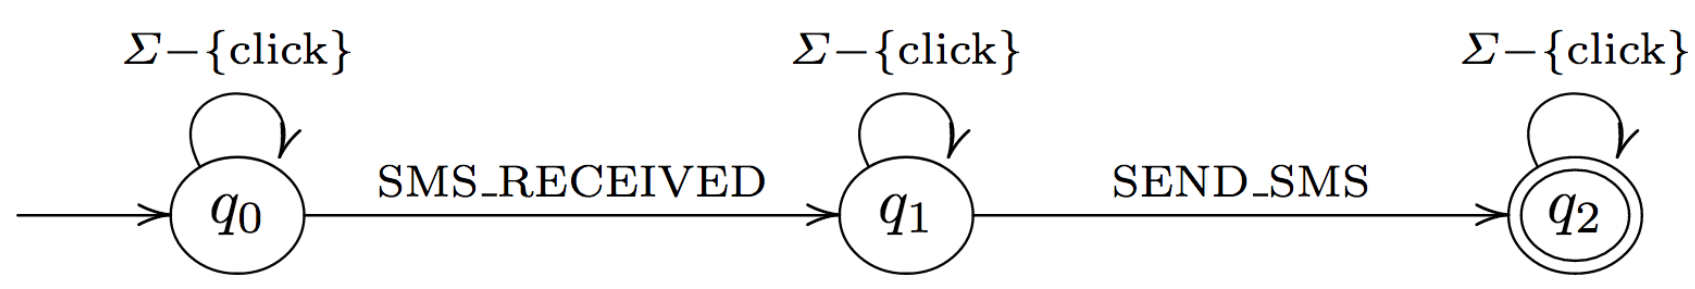
\includegraphics[width=0.8\textwidth]{Behaviourautomata.png}
%\caption{Behaviour automata of the Ggtracker family (taken from %\cite{chen2016robust})}
%\label{aut}
%\end{figure}


A \textit{behaviour automaton} is a collection  of  finite  control-sequences  of  events,  actions,  and aggregated API calls that approximates the behaviour of an application. For instance, malware behaviour of the family "Ggtracker", which immediately sends SMS to premium numbers immediately after intercepting incoming SMS, can be described by the automaton depicted in figure \ref{aut}.  $\Sigma - \{\text{click}\}$ denotes the collection of all events,  actions,  and permission-like phrases with the exception of user interactions.

A behaviour automata can be described as a collection of \textit{happen-befores}. A happen-before denotes which actions or events may follow each other in a described behaviour, such as the tuple \begin{verbatim}
(SMS_RECEIVED, SEND_SMS)
\end{verbatim}
in the mentioned example. For static analysis, the construction of tuples greater than two proved to be too expensive. However, for a dynamic analysis which we will be following, the construction of more complex tuples can be considered. 

In order to construct behaviour automata which describe the general behaviour of a program, sub-automata are generated by calculating the intersection and difference of automata obtained from observed happen-befores. 



\section{Aims and methodology}

Prof. David Aspinall and I discussed a specific project that addresses the lacking robustness of current data-centric malware detection research with a dynamic analysis approach that adapts to changes in malicious and benign applications. For that, we will rely on previous work on program behaviour abstraction using behaviour automata, as they provided promising results regarding detection robustness. 

Furthermore, instead of relying on compiled program source code, the project aims at inferring behaviour models completely from external device effects. We will primarily focus on the use of network flow logs, but the incorporation of other available data sources is possible. Malware detection without direct access to a device is particularly interesting for network providers, but also for intrusion detection in enterprise networks or in any scenario where network data is easier accessible than the devices themselves. Malware detection detached from individual devices will enable a more complete coverage in terms of protection from and localisation of intrusions.

Malware detection with behaviour based model is a quite new and promising topic and has not been used in a dynamic approach yet. Also, local malware detection in the absence of program files is an entirely new setting, in which significant progress can be achieved. 

\vspace{0.4cm}

Specifically, the project consists of two major steps:

\begin{enumerate}

\item  The first step is to build a model that identifies individual behaviour automata from a devices external effects, starting with network flow logs. This will be done dynamically with statistical methodology, i.e. incoming data streams from a device will be analysed in order to extract occurring semantic-based features. These features are then put into context with behaviour models in order to generate a stream of automata describing the behaviour of a device.

\item The second step aims at building a framework that identifies infected systems from the displayed behaviour automata. This approach will be anomaly-based rather than a direct classification into benign and malicious behaviour. Instead, we will attempt to model the spectrum of emitted behaviour automata on benign systems probabilistically, and identify anomalous activity on a device as a change point in that distribution.

\end{enumerate}

One underlying hypothesis of the project is that malicious infections can be identified just from their traces in network traffic. Since we are not looking at devices locally, behaviour automata describing purely local activity are not possible to be reconstructed. As malware relies in general heavily on network connections to achieve its specific purpose, it is expected that the differences between malware and benign software will be most pronounced in their network traffic traces, and that an accurate identification will be possible.

\subsection{Data}

Published datasets that describe external behaviour of malicious and benign devices are often given in the form of \textit{flow event logs}. A \emph{flow} is a summary of a directed connection between two computers, in which a sequence of packets are sent from a source computer to a destination computer. Flows are most often recorded as event streams in the prominent \emph{NetFlow} format by the network routers, with each \emph{flow event} typically containing a time-stamp, the duration of the connection, the IP addresses of the source, and the destination computers, the source and destination ports, the protocol of the traffic, and the number of packets and bytes sent. 

A specific dataset that will be used during this project is the CTU-13 dataset. It contains labeled NetFlow data from devices infected with 13 different types of malware. The flow events are labelled according to their origin into three groups: normal traffic from verified normal hosts, malicious traffic generated from malware, and background traffic that cannot be assigned to either one with certainty.

\subsection{Inferring behaviour automata from Network traffic}

The detection of malware from a device's external effects is a barely explored topic, and particular the involved reconstruction of behaviour models will be an entirely new approach. As mentioned above, the primary source of external traffic in our focus are network flow streams. The construction of semantic behaviour models on a device requires both the detection of isolated, point-like events such as the transmission of an e-mail as well as changes in the state of the device such as current human interaction or activity from particular applications. 

We have to consider that we will only be able to detect activity that leave traces in network flow logs (or other particular data streams we will look at). 
The identification of individual events in the network flow stream is expectedly straightforward: Flow events that show a certain signature like the use of a particular port, internet protocol or contact to a particular host can be identified as corresponding to a certain action, such as the use of port 465 corresponds to the sending of an e-mail. Actions that span over multiple flow events can be identified by looking at a rolling window consisting of fixed number of consecutive flow events, and using a classifier on feature vector spanned by the different flow events. An reasonable choice for the categorical nature of multiple flow quantities might be a decision tree classifier. The creation of happen-before-tuples can then be done by calculating the timely correlation of individual events.


The coherent estimation of device states is more complicated: Since the state of a device at one moment is highly dependent on the state it occupied before, a sequential Markovian model is a reasonable approach to the state estimation. Together with Dr. Mark Briers and Prof. Niall Adams, I recently developed an unsupervised sequential Bayesian framework that aims at inferring the presence of a user at a device and the state of usage \cite{Henrythesis2017}. The results I generated resemble the overall usage intensity of personal computers in an accurate manner, and future work on the model promises a very accurate resolution of individual task done on a device. 



The underlying model is an extended version of the \textit{Markov modulated Poisson process} and currently relies solely on the binned number of flow events during accumulation intervals. However, the model has the potential to be extended to take other flow quantities such as the flow durations or the used ports as input. 

The device state is treated as a latent Markov process $X_t$ that takes different states on a finite pre-defined state space. Observed flow events $z_i$ are generated from a tunable discrete distribution with a rate $\lambda_k$ that depends on the current state $k$ of $X_t$. From the observed flow events, we can sample directly from the the posterior distribution of $X_t$ using Gibbs sampling. 

The developed framework is fast and scalable in terms of the number of received flows. The integration of other flow quantities as input data can potentially be done in the same manner, but with continuous generator distributions where appropriate. The combined likelihood of all the input quantities will then govern the posterior distribution of $X_t$ rather than just the likelihood of $z_i$.

This framework is already capable of detecting human interaction on a device, and more work in this regard will ideally result in the distinction of individual operations acting on a device. With the trace of the device state, the construction of \textit{happen-befores} is straightforward.  

\subsection{Creating an adaptive model for anomaly discovery}

The exact design of an adaptive anomaly detecting model ultimately depends heavily on the above described automata construction performance. Therefore, it is difficult to already recommend a particular approach. 

Since we aim at creating a dynamic approach for data streams, the number of observed automata will grow continuously, and it will be impossible to extract behaviour sub-automata by looking at cross-sections and differences between all of them. Thus, the use of online methods is recommended. It is imaginable to rely on a weighting framework with more recently observed automata acquiring a higher weight, and applying intersection and difference calculation only to automata with a high enough weight. This will ensure that a possible evolution of behaviour automata is followed.


After obtaining behaviour sub-automata accordingly, the overall behaviour of benign devices has to be modelled. A specific framework I have in mind uses topic modelling to create behaviour clusters not for one device, on a remote server for all incoming data streams. Documents will be represented by batches of the incoming stream containing observed behaviour sub-automata, while words will be represented by the behaviour sub-automata. Topic modelling can then be used to observe different behaviours/topics within the incoming documents. The frequency with which specific sources target particular behaviour clusters can then be modelled with a multinomial distribution.

Multiple approaches for online topic modelling exist, both parametric \cite{NIPS2010_3902} as well as nonparametric \cite{wang2011online}. Anomalies can then be seen as deviations of incoming documents from the overall behaviour cluster distribution.

\section{Impact of the Work and summary}

The proposed project is directed towards a novel area, where significant results are achievable and will be beneficial for future research. We do not expect to build a tool that perfectly distinguishes all malware infections perfectly, but rather pave the way for more dynamic, behavioural-based detection methods in order to improve the robustness of detection methods in general. We expect that a behavioural-based approach is able to be based on the external network traffic of a device, which will allow for new possibilities regarding a wide coverage of intrusion detection. 

In order to separate significant features from background noise, our approach will rely on sophisticated statistical methods from signal processing, for which I will be a strong fit. I have successfully conducted research in the area of statistical cyber security where I produced a promising sequential method which I am preparing for publication and which I intend to use in the proposed project. Furthermore, my statistical education at Imperial College London prepared me in several areas that will be important in this project, such as hierarchical modelling, time series analysis, or statistical machine learning. 

\vspace{2cm}

\noindent I want to thank the Admission Team at the University of Edinburgh for taking the time to review my application.

\vspace{0.6cm}
\noindent Henry Clausen
\pagebreak

\bibliography{sample}
\bibliographystyle{plain}


\end{document}
